



%
%
%
%
%
%





\begin{figure}[t]
	\center
	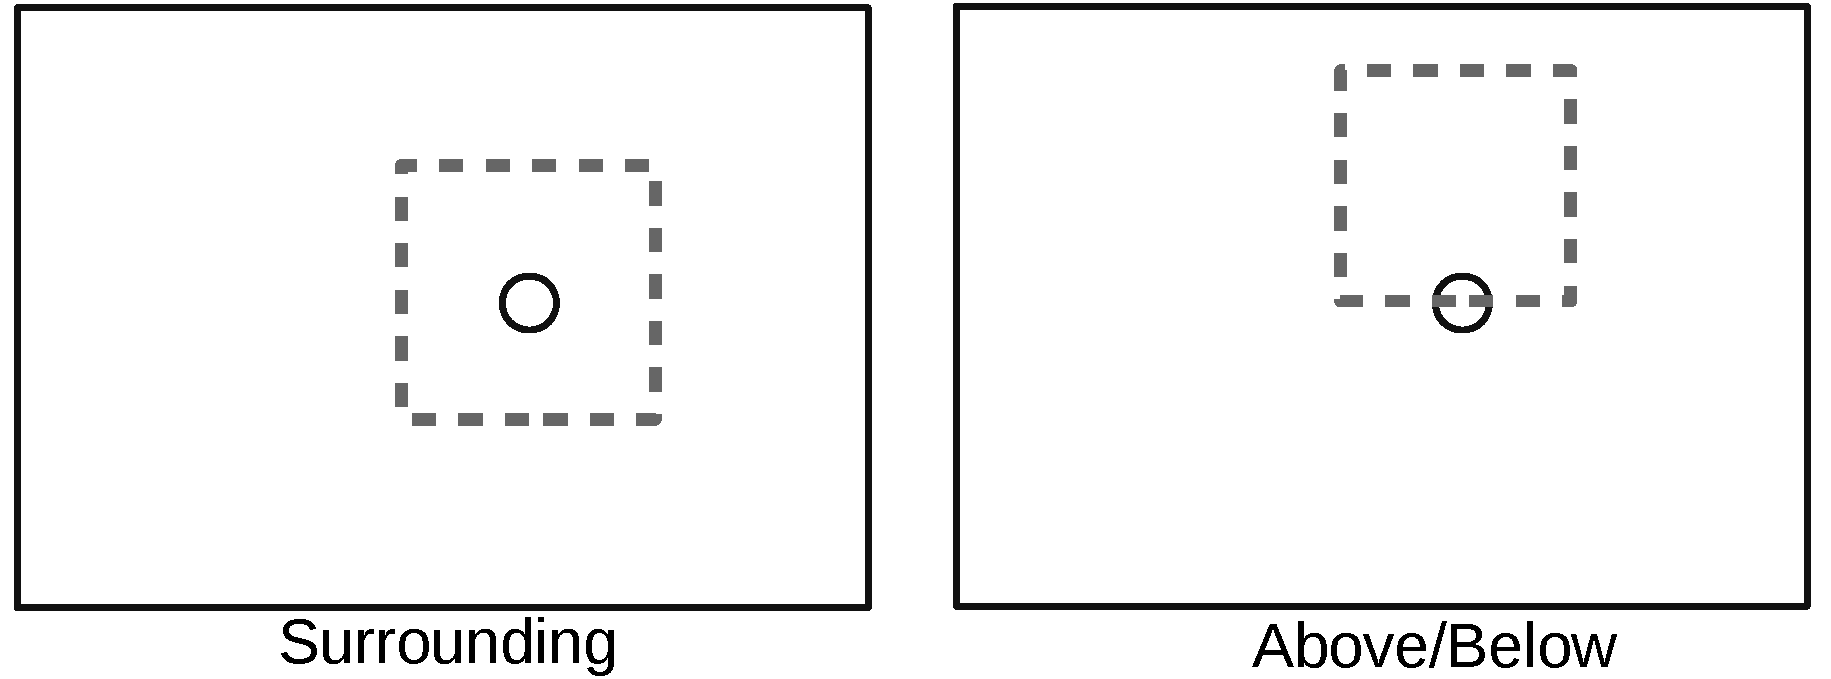
\includegraphics[width=.8\linewidth]{./figs/pairwise_conn}
\caption{An illustration of constructing pairwise connections in a CRF graph.
A node is connected to all other nodes which lie within the range box (dashed box in the figure).
Two types of spatial relations are described in the figure, which
correspond to two types of pairwise potential functions.
}
\label{fig:pairwise}
\end{figure}











\section{Modeling semantic pairwise relations}

Fig.~\ref{fig:potential_net} conceptualizes our architecture at a high level.
%
Given an image, we first apply a convolutional network to generate a feature map.
We refer to this network as `FeatMap-Net'.
The resulting feature map is at a lower resolution than the original image because of the down-sampling operations in the pooling layers.
%

We then create the CRF graph as follows:
for each location in the feature map (which corresponds to a rectangular region in the input image) we create one node in the CRF graph.
%
%
Pairwise connections in the CRF graph are constructed by connecting one node to all other nodes 
which lie within a spatial range box (the dashed box in Fig.~\ref{fig:pairwise}).
We consider different spatial relations by defining different types of range box, and each type of spatial relation is modeled by a specific pairwise potential function.
As shown in Fig.~\ref{fig:pairwise},  our method models the ``surrounding" and ``above/below" spatial relations.
%
%
In our experiments, the size of the range box (dash box in the figure) size is $0.4a \times 0.4a$.
Here we denote by $a$ the length of the short edge of the feature map.


Note that although `FeatMap-Net' defines a common architecture, in fact we train three such networks: one for the unary potential and one each for the two types of pairwise potential.




\section{Contextual Deep CRFs}
\label{sec:crf_details}

Here we describe the details of our deep CRF model.
We denote by $\x \in \cX$ one input image and $\y \in \cY$ the labeling mask which describes the label configuration of each node in the CRF graph.
The energy function is denoted by $E(\y, \x; \btheta)$ which models the compatibility of the input-output pair, with a small output value indicating high confidence in the prediction $\y$.
All network parameters are denoted by $\btheta$ which we need to learn.
The conditional likelihood for one image is formulated as follows:
\begin{equation}\label{eq:prob}
\begin{aligned}
\small
\Prr(\y|\x) = \frac{1}{Z(\x)} \exp [- E(\y, \x)].
\end{aligned}
\end{equation}
%
%
%
%
%
%
Here $Z(\x) = \sum_{\y} \exp [ -E(\y, \x) ]$ is the partition function.
The energy function is typically formulated by a set of unary and pairwise potentials:
\begin{align}
\label{eq:energy}
\small
	E(\y, \x) = &  \sum_{U \in \cU} \sum_{p \in \cN_U } U(y_{p}, \x_p) %
  + \sum_{V \in \cV} \sum_{(p,q) \in \cS_V} V(y_{p}, y_{q}, \x_{pq}). \notag
\end{align}
Here $U$ is a unary potential function,
and to make the exposition more general, we consider multiple types of unary potentials with
$\cU$ the set of all such unary potentials.
$\cN_U$ is a set of nodes for the potential $U$.
Likewise, $V$ is a pairwise potential function
 with $\cV$ the set of all types of pairwise potential. $\cS_V$ is the set of edges for the potential $V$.
$\x_{p}$ and $\x_{pq}$  indicates the corresponding image regions which associate to the specified node and edge.












\begin{figure}[t]
	\centering
	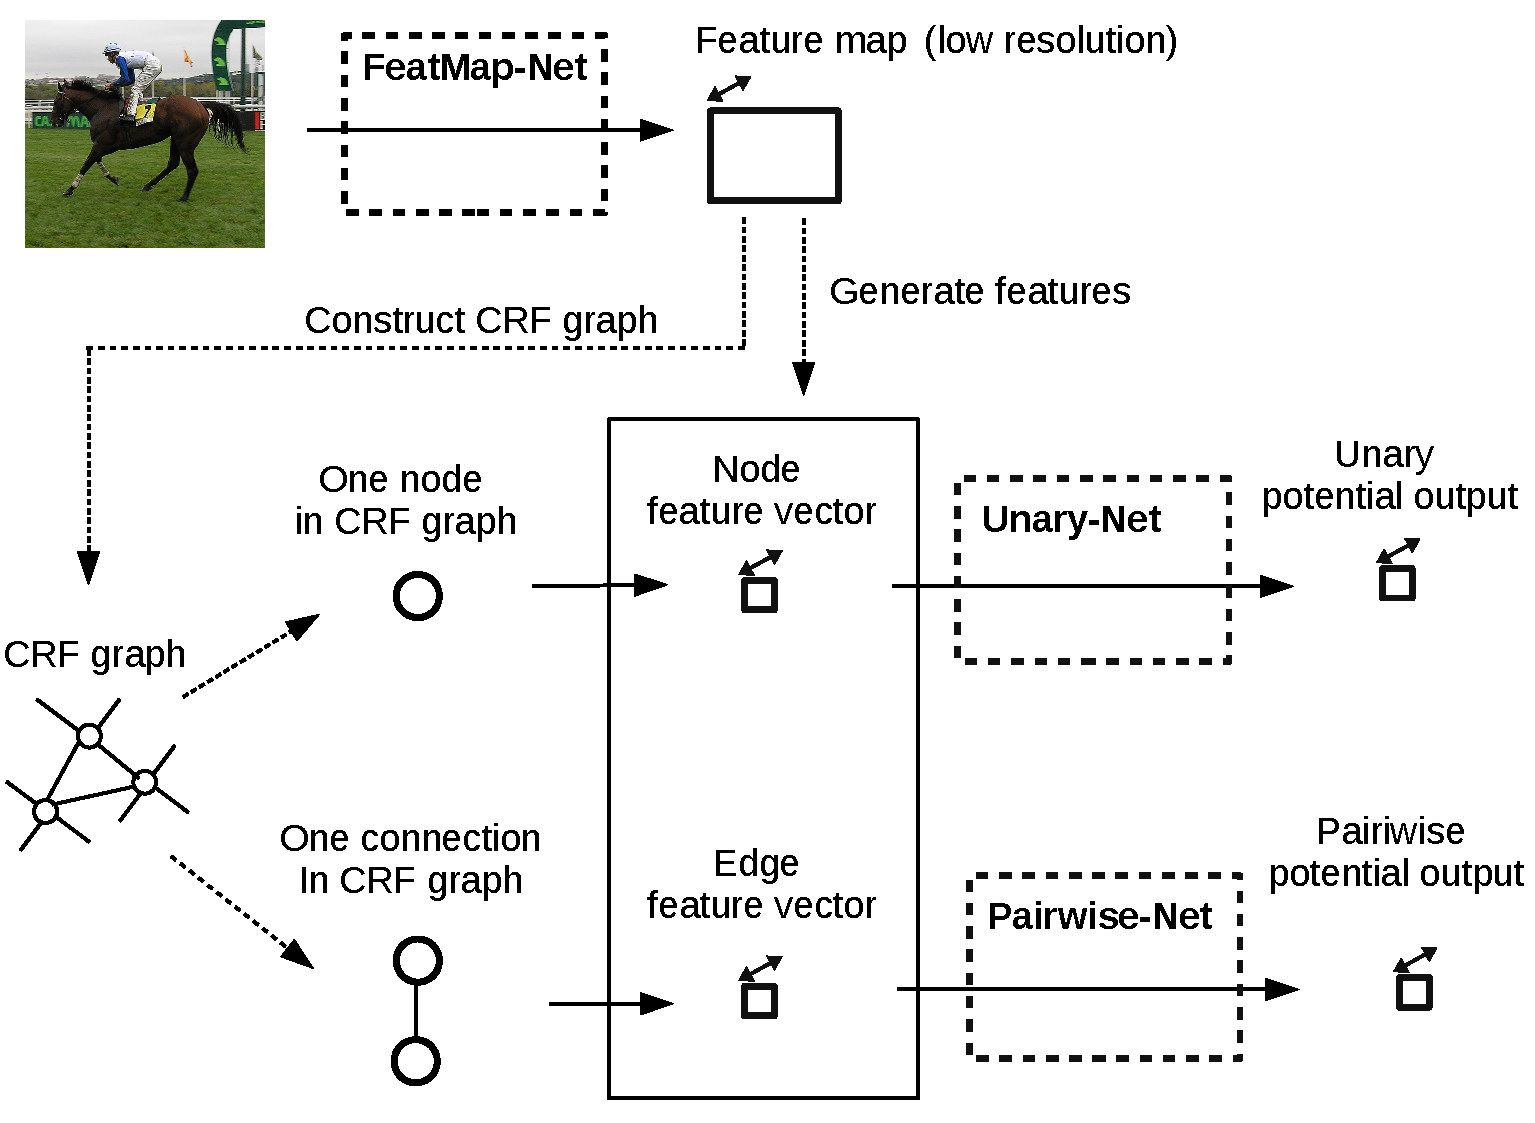
\includegraphics[width=1\linewidth]{./figs/potential_net}
\caption{An illustration of generating unary or pairwise potential function outputs.
First a feature map is generated by a FeatMap-Net, and a CRF graph is constructed based on the spatial resolution of the feature map.
Finally the Unary-Net (or Pairwise-Net) produces potential function outputs.}
\label{fig:potential_net}
\end{figure}





\begin{figure*}[t]
	\center
	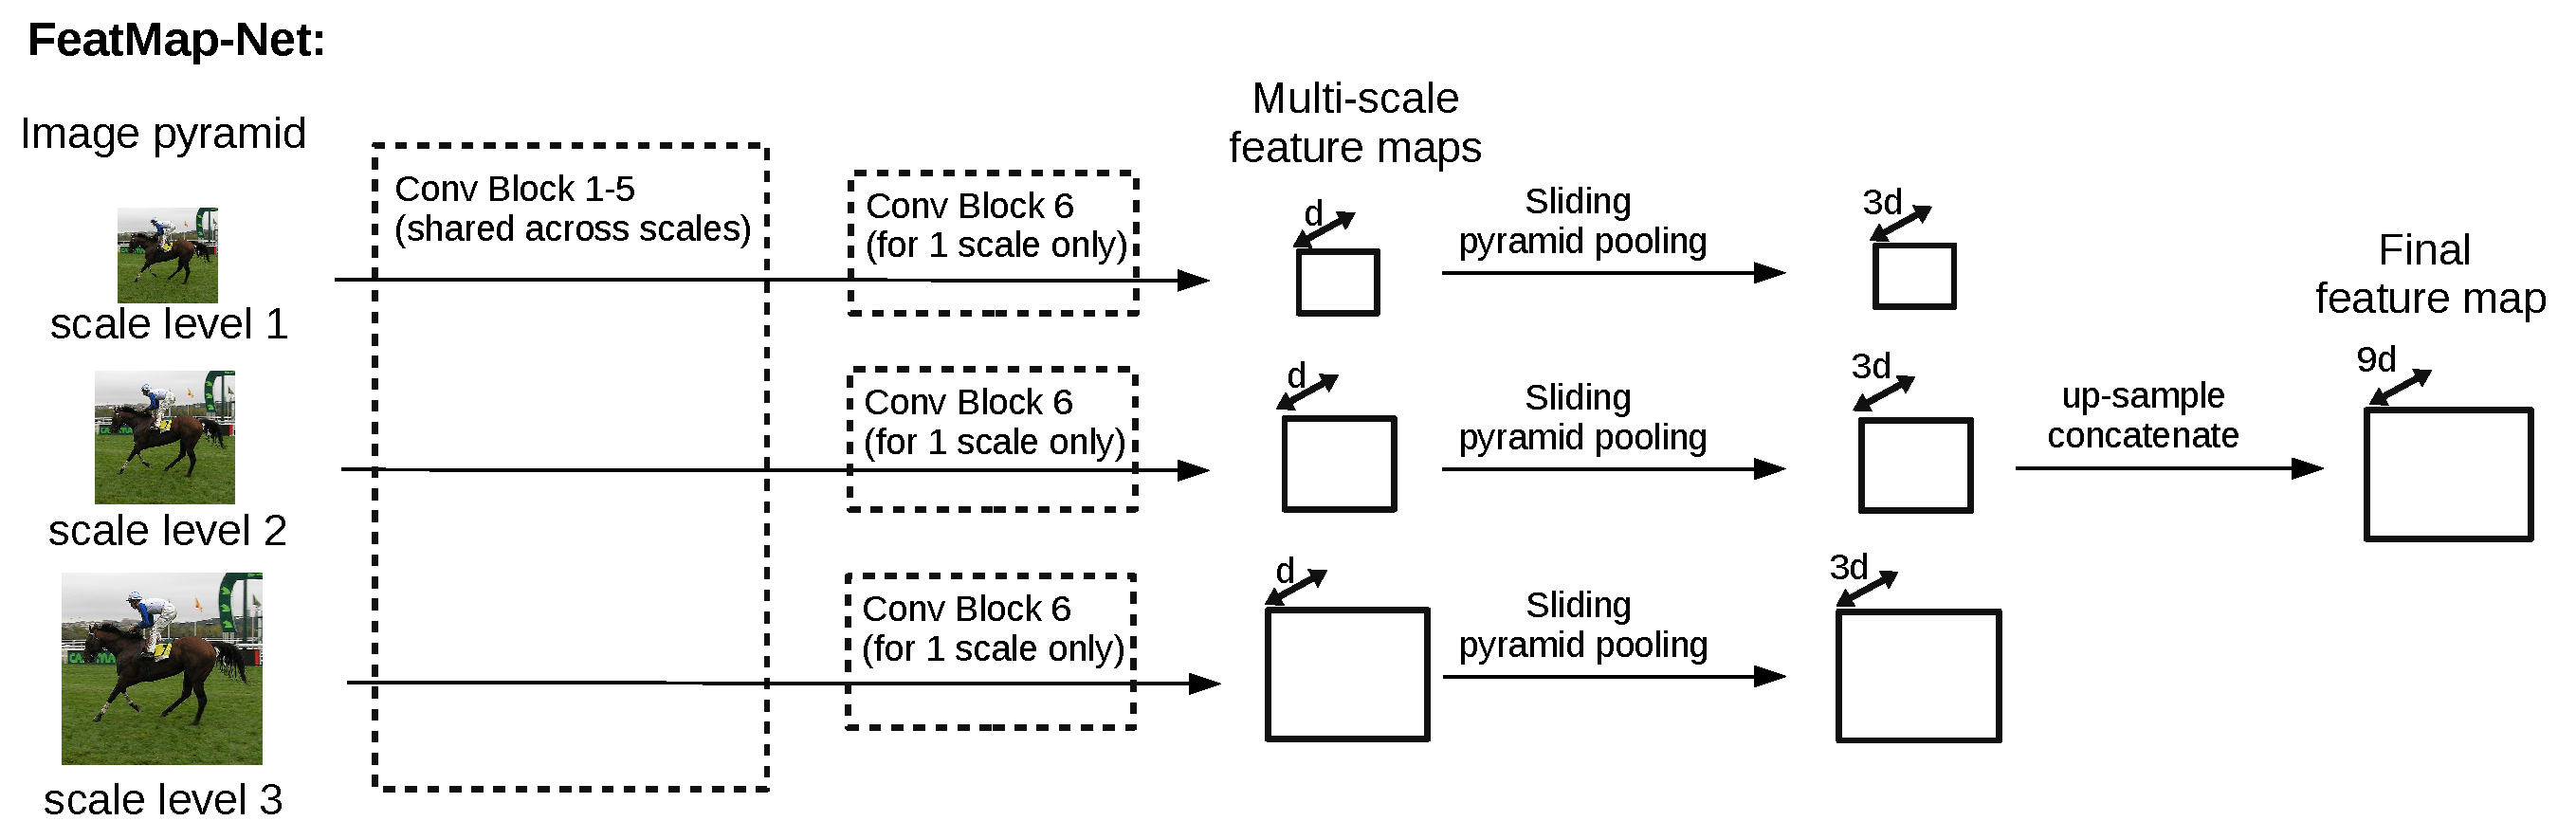
\includegraphics[width=.9\linewidth]{./figs/dense_cnn2}
\caption{The details of our FeatMap-Net.
An input image is first resized into $3$ scales,
then each resized image goes through 6 convolution blocks to output one feature map.
Top $5$ convolution blocks are shared for all scales. Every scale has a specific convolution block (Conv Block 6).
We perform $2$-level sliding pyramid pooling (see Fig.~\ref{fig:pooling} for details).
%
$d$ indicates the feature dimension.
}
\label{fig:featmapnet}
\end{figure*}







\subsection{Unary potential functions}
We formulate the unary potential function by stacking the FeatMap-Net for generating feature maps and 
a shallow fully connected network (referred to as Unary-Net) to generate the final output of the unary potential function.
The unary potential function is written as follows:
\begin{equation}
	U(y_{p}, \x_p; \btheta_U) = - z_{p,y_p} (\x; \btheta_U).
\end{equation}
Here $z_{p, y_p }$ is the output value of Unary-Net, which corresponds to the $p$-th node and the $y_p$-th class.


Fig.~\ref{fig:potential_net} includes an illustration of the Unary-Net and how it integrates with FeatMap-Net.
%
The unary potential at each CRF node is simply the $K$-dimensional output (where $K$ is the number of classes) of Unary-Net applied to the node feature vector from the correpsonding location in the feature map (i.e. the output of FeatMap-Net).
%
%





\subsection{Pairwise potential functions}
Fig. \ref{fig:potential_net} likewise illustrates how the pairwise potentials are generated.  The edge features are formed by concatenating 
the corresponding feature vectors of two connected nodes (similar to~\cite{kolesnikov2014closed}).  The feature vector for each node in the pair is from the feature map output by FeatMap-Net. The edge features of one pair  are then fed to a shallow fully connected network (referred to as Pairwise-Net) to generate the final output that is the pairwise potential.  The size of this is $K \times K$ to match the number of possible label combinations for a pair of nodes. 
The pairwise potential function is written as follows:
\begin{align}
	V & (y_{p}, y_{q},  \x_{pq}; \btheta_V) = - z_{p, q, y_p, y_q} (\x; \btheta_V).
\end{align}
Here $z_{p, q,  y_p,  y_q }$ is the output value of Pairwise-Net.
It is the confidence value for the node pair $(p, q)$ when they are labeled with the class value $( y_p,  y_q )$, which measures the compatibility of the label pair $(y_{p}, y_{q}$) given the input image $\x$.
$\btheta_V$ is the corresponding set of CNN parameters for the potential $V$, which we need to learn.


%
%
%
%
%
%




Our formulation of pairwise potentials is different from the Potts-model-based formulation in the existing methods of \cite{ChenPKMY14,zheng2015conditional}.
The Potts-model-based pairwise potentials are a log-linear functions and
employ a special formulation for enforcing neighborhood smoothness.
In contrast, our pairwise potentials model the semantic compatibility between two nodes
 with the output for every possible value of the label pair $(y_{p}, y_{q}$) individually parameterized by CNNs. 


In our system, after obtaining the coarse level prediction, we still need to perform a refinement step to obtain the final high-resolution prediction 
(as shown in Fig.~\ref{fig:general_graph}).
Hence we also apply the dense CRF method \cite{krahenbuhl2012efficient}, as in many other recent methods, in the prediction refinement step.
Therefore, our system takes advantage of both contextual CNN potentials and the traditional smoothness potentials to improve the final system.
More details are described in Sec.~\ref{sec:prediction}.









As in \cite{winn2006layout,heesch2010markov},
modeling asymmetric relations requires the potential function is capable of modeling input orders, 
since we have: $ V  (y_{p}, y_{q},  \x_{pq}) \neq V (y_{q}, y_{p},  \x_{qp})$.
Take the asymmetric relation ``above/below" as an example;
we take advantage of the input pair order to indicate the spatial configuration of two nodes,
thus the input $(y_p, y_q, \x_{pq})$
indicates the configuration that the node $p$ is spatially lies above the node $q$.

The asymmetric property is readily achieved with our general formulation of pairwise potentials.  
The potential output for every possible pairwise label combination for $(p,q)$ is individually parameterized by the pairwise CNNs.  



























\section{Exploiting background context}
\label{sec:network_details}

To encode rich background information,
we use multi-scale CNNs and  sliding pyramid pooling \cite{lazebnik2006beyond} for our FeatMap-Net.
Fig.~\ref{fig:featmapnet} shows the details of the FeatMap-Net.


CNNs with multi-scale image network inputs have shown good performance in some recent segmentation methods \cite{farabet2013learning,MostajabiYS14}.
The traditional pyramid pooling (in a sliding manner) on the feature map is able to capture information from background regions of different sizes.
%
We observe that these two techniques (multi-scale network design and pyramid pooling) 
for encoding background information are very effective for improving performance.



Applying CNNs on multi-scale images has shown good performance in some recent segmentation methods \cite{farabet2013learning,MostajabiYS14}.
In our multi-scale network, an input image is first resized into $3$ scales,
then each resized image goes through 6 convolution blocks to output one feature map.
In our experiment, the $3$ scales for the input image are set to $1.2$, $0.8$ and $0.4$.
All scales share the same top $5$ convolution blocks.
In addition, each scale has an exclusive convolution block (``Conv Block 6" in the figure) 
which captures scale-dependent information.
The resulting $3$ feature maps (corresponding to $3$ scales) are of different resolutions, therefore we  upscale the two smaller ones to the size of the largest feature map using bilinear interpolation. These feature maps are then concatenated to form one feature map.


We perform spatial pyramid pooling \cite{lazebnik2006beyond} (a modified version using sliding windows) 
on the feature map to capture information from background regions in multiple sizes.
This increases the field-of-view for the feature map and thus it is able to capture the information from a large image region.
Increasing the field-of-view generally helps to improve performance \cite{ChenPKMY14}.


The details of spatial pyramid pooling are illustrated in Fig. \ref{fig:pooling}.
In our experiment, we perform $2$-level pooling for each image scale.
We define $5 \times 5$ and $9 \times 9$ sliding pooling windows (max-pooling) to generate $2$ sets of pooled feature maps,
which are then concatenated to the original feature map to construct the final feature map.


The detailed network layer configuration for all networks are described in Fig.~\ref{fig:network_conf}.
%









\begin{figure}[t]
	\center
	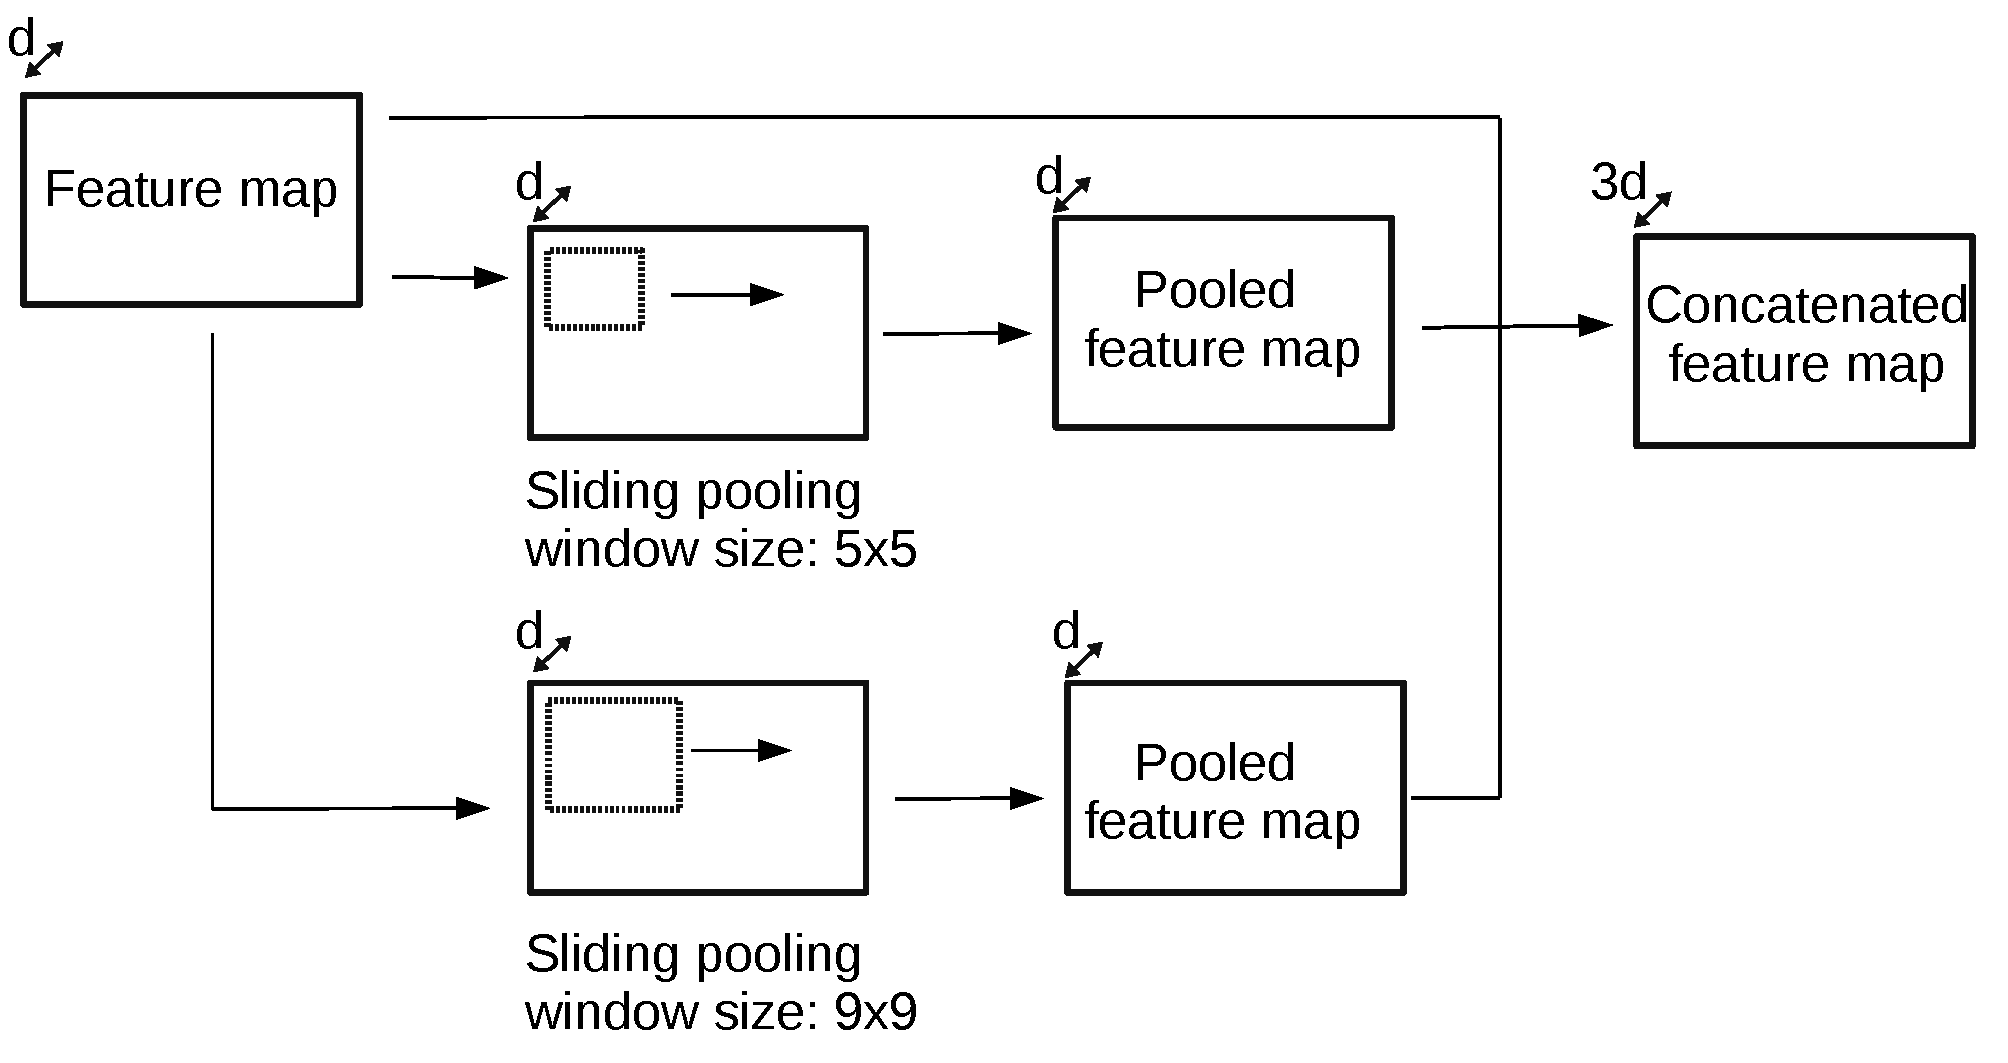
\includegraphics[width=1\linewidth]{./figs/pooling}
\caption{
Details for sliding pyramid pooling.
We perform $2$-level sliding pyramid pooling on the feature map for capturing patch-background context, 
which encode rich background information and increase the field-of-view for the feature map.
}
\label{fig:pooling}
\end{figure}






\begin{figure}[t]
	\center
	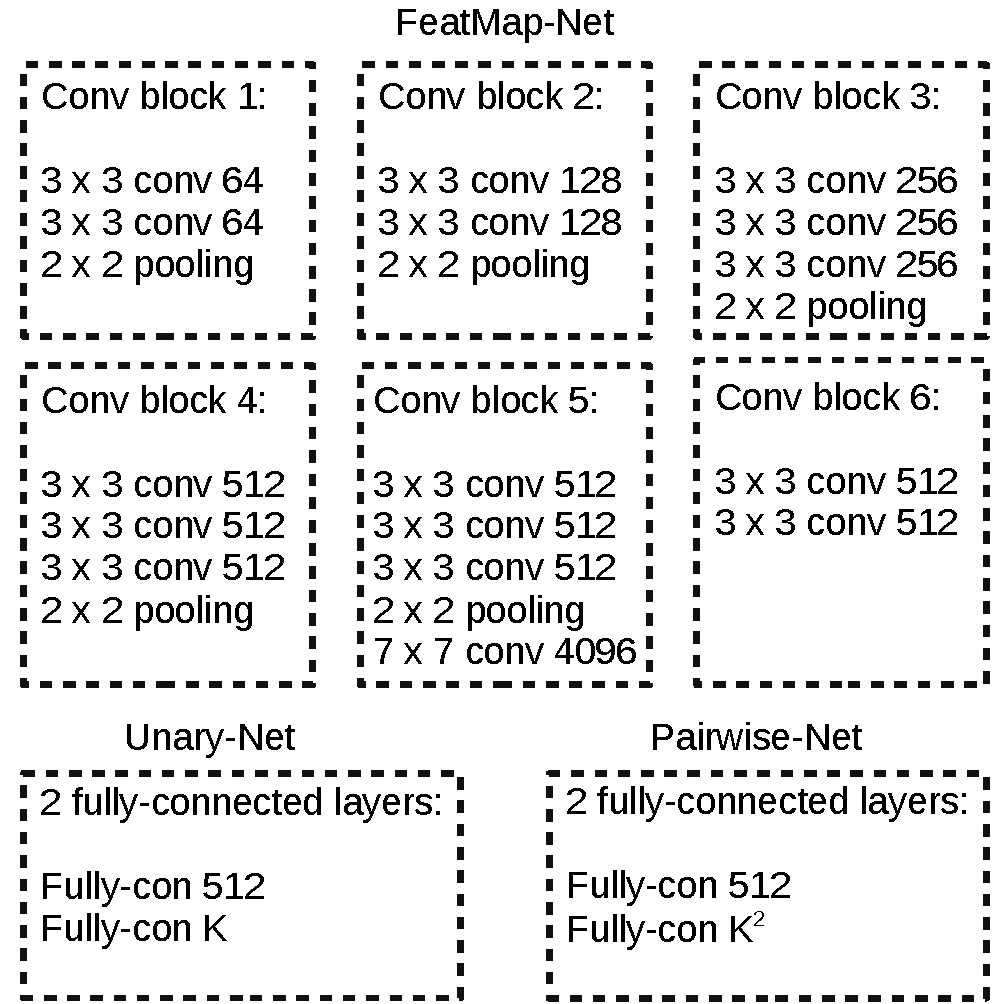
\includegraphics[width=.75\linewidth]{./figs/network_layers}
\caption{The detailed configuration of the networks: FeatMap-Net, Unary-Net and Pairwise-Net.
  $K$ is the number of classes.
  For FeatMap-Net, the top 5 convolution blocks share the same configuration
as the convolution blocks in the VGG-16 network. The stride of the last max pooling layer is 1, and
for the other max pooling layers we use the same stride setting as VGG-16.
}
\label{fig:network_conf}
\end{figure}







\section{Prediction}
\label{sec:prediction}

In the prediction stage,
our deep structured model will generate low-resolution prediction (as shown in Fig.~\ref{fig:general_graph}), 
which is $1/16$ of the input image size.
This is due to the stride setting of pooling or convolution layers for sub-sampling.
Therefore, we apply two prediction stages for obtaining the final high-resolution prediction: 
the coarse-level prediction stage and the prediction refinement stage.


\subsection{Coarse-level prediction stage}
We perform CRF inference on our contextual structured model to obtain the coarse prediction of a test image.
We consider the marginal inference over nodes for prediction:
\begin{align} \label{eq:inference}
\forall p \in \cN: \;\; \Prr(y_p|\x)&= {\textstyle \sum_{\y \backslash y_p } \Prr(\y|\x)}.
\end{align}
The obtained marginal distribution can be further applied in the next prediction stage for boundary refinement.

Our CRF graph does not form a tree structure,
nor are the potentials submodular,
hence we need to an apply approximate inference.
To address this we
apply an efficient  message passing algorithm which is based on the mean field approximation \cite{Nowozinstruct}.
The mean field algorithm constructs a simpler distribution $Q(\y)$, e.g.,
a product of independent marginals: 
$Q(\y)=\prod_{p \in \cN} Q_p (y_p)$, 
which minimizes the KL-divergence between the distribution $Q(\y)$ and $\Prr(\y)$.
In our experiments, we perform $3$ mean field iterations.


\subsection{Prediction refinement stage}
We generate the score map for the coarse prediction from the marginal distribution which we obtain from the mean-field inference.
We first bilinearly up-sample the score map of the coarse prediction to the size of the input image.
Then we apply a common post-processing method \cite{krahenbuhl2012efficient} (dense CRF)
to sharpen the object boundary for generating the final high-resolution prediction.
This post-processing method leverages low-level pixel intensity information (color contrast) for boundary refinement. 
Note that most recent work on image segmentation similarly produces low-resolution prediction
 and have a upsampling and refinement process/model for the final prediction, e.g., 
\cite{ChenPKMY14,zheng2015conditional,Dai2015arXiv}.

In summary, we simply perform bilinear upsampling of the coarse score map and apply the boundary refinement post-processing.
We argue that this stage can be further improved by applying more sophisticated refinement methods, e.g., training deconvolution networks \cite{noh2015learning}, 
training multiple coarse to fine learning networks \cite{eigen2015predicting}, 
and exploring middle layer features for high-resolution prediction \cite{hariharan2014hypercolumns,LongSD14}.
It is expected that applying better refinement approaches will gain further performance improvement.












\section{CRF training}

A common approach for CRF learning is to maximize the likelihood,
or equivalently minimize the negative log-likelihood, which can be written
for one image as:
\begin{align}
 - \log \Prr(\y | \x; \btheta) = E(\y, \x; \btheta) + \log Z(\x; \btheta).
\label{eq:Prr}
\end{align}
Adding regularization to the CNN parameter $\btheta$, the optimization problem for CRF learning is: 
{\small
\begin{align}
\label{eq:crf_learning_org}
\min_{\btheta} \frac{\lambda}{2} \fnorm \btheta + \sum_{i=1}^N \biggr[ E(\y^{(i)}, \x^{(i)}; \btheta) + \log Z(\x^{(i)}; \btheta) \biggr].
\end{align}
}
%
%
%
%
Here $\x^{(i)}$, $\y^{(i)}$ denote the $i$-th training image and its segmentation mask; $N$ is the number of training images; $\lambda$ is the weight decay parameter.
%
%
%
%
%
%
%
We can apply stochastic gradient (SGD) based methods to optimize the above problem for learning $\btheta$.
The energy function $E (\y, \x; \btheta)$ is constructed from CNNs, and its
gradient $\gradient_\btheta E (\y, \x; \btheta)$ easily computed
by applying the chain rule as in conventional CNNs.
However, the partition function $Z$ brings difficulties for optimization.  Its gradient is:
\begin{align}
\gradient_\btheta  \log &  Z(\x ; \btheta)  \notag  \\
	 = &  \sum_\y \frac{\exp[-E(\y, \x; \btheta)]} {\sum_{\y'} \exp[-E(\y', \x; \btheta)]} \gradient_\btheta [ - E (\y, \x; \btheta)] \notag \\
	 = &  - \expect_{\y \sim \Prr(\y | \x ; \btheta)} \gradient_\btheta E (\y, \x; \btheta)
\end{align}
Generally the size of the output space $\cY$
is exponential in
the number of nodes, which prohibits the direct calculation of $Z$ and its gradient.
The CRF graph we considered for segmentation here is a loopy graph (not tree-structured),
for which the inference is generally computationally expensive.
More importantly, usually a large number of SGD iterations (tens or hundreds of thousands) are required for
training CNNs. Thus performing inference at each SGD iteration is very computationally expensive.




\subsection{Piecewise training of CRFs}


Instead of directly solving the optimization in \eqref{eq:crf_learning_org},
we propose to apply an approximate CRF learning method.
In the literature,
there are two popular types of learning methods which approximate the CRF objective
: pseudo-likelihood learning \cite{besag1977efficiency} and piecewise learning \cite{SuttonM05}.
The main advantage of these methods  in term of training deep CRF is that they  do not involve marginal inference for gradient calculation,
which significantly improves the efficiency of training.
Decision tree fields \cite{NowozinRBSYK11} and regression tree fields \cite{jancsary2012regression}
are based on pseudo-likelihood learning, while
piecewise learning has been applied in the work \cite{SuttonM05,kolesnikov2014closed}.

Here we develop this idea for the case of training the CRF with the CNN potentials.
In piecewise training, 
the conditional likelihood 
is formulated as a number of independent likelihoods defined on potentials, written as:
\begin{align}
\Prr (\y | \x) = \prod_{U \in \cU} \prod_{ p \in \cN_{U}} \Prr_{U} ( y_p | \x) \prod_{V \in \cV}
\prod_{ (p,q) \in \cS_{V}} \Prr_{V} ( y_p, y_q | \x). \notag
\end{align}
The likelihood $\Prr_{U} ( y_p | \x)$ is constructed from the unary potential $U$.
Likewise, $\Prr_{V} ( y_p, y_q | \x)$ is constructed from the pairwise potential $V$.
$\Prr_{U}$ and $\Prr_{V}$ are written as:
\begin{align}
\Prr_{U}(y_p|\x) &  = \frac{\exp [- U(y_p, \x_p)]}{\sum_{y'_p} \exp [ -U(y'_p, \x_p) ]}, \label{eq:pu} \\
\Prr_{V}(y_p, y_q|\x) &  = \frac{\exp [- V(y_p, y_q, \x_{pq})]}{\sum_{y'_p, y'_q} \exp [ -V(y'_p, y'_q, \x_{pq}) ]}
\label{eq:pv}.
\end{align}
 Thus the optimization for piecewise training is to minimize
 the negative log likelihood with regularization:
\begin{align}
	\min_{\btheta} \frac{\lambda}{2} & \fnorm \btheta -
	 \sum_{i=1}^N \biggr[ \sum_{U \in \cU}
		\sum_{ p \in \cN_{U}^{(i)}} \log \Prr_{U} ( y_p | \x^{(i)}; \btheta_U) \notag \\
	& + \sum_{V \in \cV} \sum_{ (p,q) \in \cS_{V}^{(i)}} \log \Prr_{V} ( y_p, y_q | \x^{(i)}; \btheta_V) \biggr].
	\label{eq:partitioned}
\end{align}
Compared to the objective in \eqref{eq:crf_learning_org} for direct maximum likelihood learning,
the above objective does not involve the global partition function $Z(\x ; \btheta)$.
To calculate the gradient of the above objective,
we only need to calculate the gradient
$\gradient_{\btheta_U} \log \Prr_{U}$
and
$\gradient_{\btheta_V} \log \Prr_{V}$.
With the definition in \eqref{eq:pu}, $\Prr_{U}$ is a conventional Softmax normalization function over only $K$ (the number of classes) elements. 
Similar analysis can also be applied to $\Prr_{V}$.
Hence, we can easily calculate the gradient without involving expensive inference.
Moreover, we are able to perform parallel training of potential functions, since the above objective is formulated as a summation of independent log-likelihoods.

 As previously discussed, CNN training usually involves a large number of gradient update iterations.  However this means that expensive inference during every gradient iteration becomes impractical.  Our piecewise approach here provides a practical solution for learning CRFs with CNN potentials on large-scale data.





